\chapter{Proposal}
\label{ch.proposal}

The proposal for this undergraduate dissertation is made up of two main contributions.
The first contribution will be the port of the \textit{Inter-Cluster Communication Module},
described in Section \ref{sec.inter-cluster-communication}, for the \mppa manycore processor.
The second contribution will be the design and implementation of communication services
of a master-slave \os, described in Section \ref{sec.communication-services}, on top of
the communication module.

\section{Inter-Cluster Communication Module}

	Ideally, the \hal implementation should not use any other layer of software to
	deal with the hardware. However, the implementation of \hal in \mppa uses the
	software stack made available by Kalray.
	In order to replace them, a great effort would be necessary, fleeing the proposal
	of this work and the scope of Pedro H. Penna's Ph.D.
	The main reasons for this decision were due to poor documentation and the
	inability to execute kernel mode code freely.

	\begin{figure}[t]
		\centering
		\caption{Software Stack of the \mppa.}

		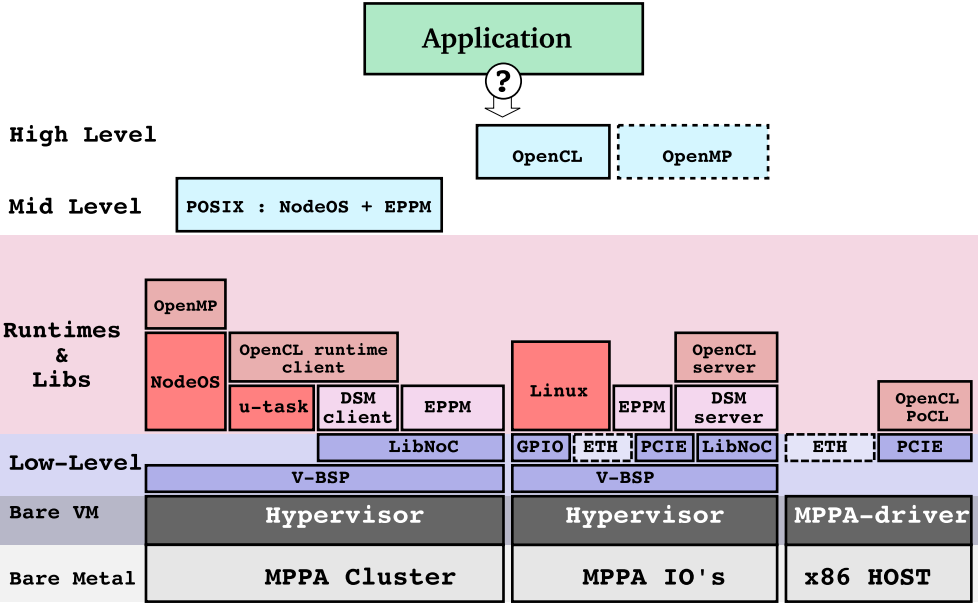
\includegraphics[width=.7\textwidth]{images/software-stack.png}

		Source: \mppa Processor Documentation.

		\label{fig.software-stack}
	\end{figure}

	Figure \ref{fig.software-stack} shows the software stack present for the \mppa.
	From it, only the \textit{hypervisor} and the \textit{vbsp} library will be used.
	The hypervisor is used to virtualize the hardware by separating it into logical
	parts, e.g., core virtualization, \cnoc virtualization, and \dnoc virtualization.
	It also exports routines to manage, configure, and allow access to virtual resources.
	The vbsp library, in turn, provides primitives for setting interrupts.

	The inter-cluster communication module will use \hal's interfaces and the
	virtualizations of the \cnoc and \dnoc interfaces directly.
	Virtual \noc interfaces export asynchronous calls to acquire read and write
	permission from registers that configure the hardware for a given task.
	For instance, the \dma configuration for asynchronous sending is abstracted by
	$\mu$threads that are configured through global structures provided by the hypervisor.

	\begin{table}[t]
		\caption{Cluster Identification.}

		\begin{tabular}{|l|l|l|}
			\hline
						         & \textbf{Physical ID} & \textbf{Logical ID} \\ \hline
			\textbf{\ccluster}   & 0-15                 & 0-15                \\ \hline
			\textbf{\iocluster0} & 128-131              & 16-19               \\ \hline
			\textbf{\iocluster1} & 192-195              & 20-23               \\ \hline
		\end{tabular}

		\label{tab.cluster-id}
	\end{table}

	Clusters have two identifiers, one physical (physical ID) and the
	other logical (logical ID).
	The physical ID's are the numbers in hardware that identically them
	during the process of routing the data through \noc.
	The logical ID's are numbers associated with the physical ID's so
	that it is possible to identify the clusters outside the \hal.
	Logical ID's primarily serve to disassociate the cluster
	identification from the architecture in which \hal is implemented.
	Table \ref{tab.cluster-id} shows the physical and logical
	identification performed for \mppa.

	\begin{table}[]
		\caption{Partitions of \noc resources by abstraction.}

		\begin{tabular}{l|l|l|l|l|}
			\cline{2-5}
										   & \multicolumn{2}{c|}{\textbf{\cnoc}} & \multicolumn{2}{c|}{\textbf{\dnoc}} \\ \cline{2-5}
										            & \textbf{RX Slot} & \textbf{TX Channel} & \textbf{RX Slot} & \textbf{TX Channel} \\ \hline
			\multicolumn{1}{|l|}{\textbf{\mailbox}} & 0-23             & 0                   & 0-23             & 1-3                 \\ \hline
			\multicolumn{1}{|l|}{\textbf{\portal}}  & 24-47            & 1-2                 & 24-47            & 4-7                 \\ \hline
			\multicolumn{1}{|l|}{\textbf{\sync}}    & 48-71            & 3                   & -                & -                   \\ \hline
		\end{tabular}

		\label{tab.noc-resources}
	\end{table}

	To perform the communication between two clusters, it is necessary that the
	sender knows which resource the receiver will use.
	For this reason, the receive slot range of \cnoc and \dnoc are partitioned
	by abstraction, as can be seen in Table \ref{tab.noc-resources}.
	Within a partition, each slot is associated with a cluster's logical ID.
	On the other hand, the transmitters use sending channels that need to
	be reserved during the entire operation.
	Thus, Table \ref{tab.noc-resources} also shows the partition of the
	sending channels for each abstraction.

	\subsection{Sync}

\begin{figure}[t]
\begin{lstlisting}[
	caption=HAL Sync Interface for Receiver Cluster,
	label=code:sync-receiver,
]
	/* @brief Allocates and configures the receiving side of
	 *        the synchronization point.                     */
	int sync_create(const int *nodes, int nnodes, int type);

	/* @brief Releases and cleans receiver buffer. */
	int sync_unlink(int syncid);

	/* @brief Wait signal on a specific synchronization point. */
	int sync_wait(int syncid);
\end{lstlisting}
\end{figure}

\begin{figure}[t]
\begin{lstlisting}[
	caption=HAL Sync Interface for Sender Cluster,
	label=code:sync-sender,
]
	/*  @brief Allocates and configures the sending side of
	 *  the synchronization point.                          */
	int sync_open(void);

	/* @brief Releases the sender resources on a specific DMA channel. */
	int sync_close(int syncid);

	/* @brief Send signal on a specific synchronization point. */
	int sync_signal(int syncid, const int *nodes, int nnodes, int type);
\end{lstlisting}
\end{figure}

		As described in Section \ref{sec.sync-abs}, the \sync abstraction allows the
		creation of distributed barriers.
		The \sync can be decomposed into two sets of functions, where the
		Code \ref{code:sync-receiver} shows the functions to one clusters
		that will receive signals, and Code \ref{code:sync-sender} shows the
		ones that will send.
		Each set allocates different types of resources.
		Accurately, the receiver must allocate a receive slot of the frame,
		and the transmitter will allocate a transmitter channel of the frame.
		Because of this, 24 synchronization points can be created (\texttt{sync\_create()}),
		and only 1 can be opened (\texttt{sync\_open()}) per cluster.

		Sync Functions implement two different types, depending on who cluster
		should be the master of the synchronization operation.
		Specifically, every synchronization operation is separated into a
		master cluster and one or more slave clusters defined by the
		\texttt{ONE\_TO\_ALL} and \texttt{ALL\_TO\_ONE} constants.
		The master always takes the role "ONE" and the slaves the "ALL" role.
		The following subsections describe the behavior and implementation
		details of each type of synchronization.

			\subsubsection*{\texttt{ONE\_TO\_ALL} Synchronization Type}

				The slave clusters involved in this type of synchronization expect
				a signal sent from the master.
				To do this, each slave will perform the function \texttt{sync\_create()}
				by allocating the resource associated with the master's logical ID.
				After allocating and configuring the resource, the cluster can
				continue to run without worrying about whether the signal was received.
				When the time comes to perform the synchronization, it is enough for
				the slave to run the function.
				Upon receiving the signal, the sync will auto reconfigure the resource
				and free the cluster.

				The cluster master, in turn, must perform the complementary functions.
				That is, first, the master will allocate a sending resource by calling
				the \texttt{sync\_open()} function.
				After that, it should inform the set of clusters that will receive the
				signal on its logical ID.
				Finally, both can release sync resources by calling release functions,
				\texttt{sync\_unlink()} for the slave and \texttt{sync\_close()} to
				the master.

			\subsubsection*{\texttt{ALL\_TO\_ONE} Synchronization Type}

				Analogously to the previous type, the only changes are just on
				the roles in which they are reversed.
				The master must perform the functions of creation, configuration
				of the resources, and waiting for the numerous signals.
				The resource allocated by the master must be the resource
				associated with its logical ID.
				On the other hand, the slaves will perform the functions of
				opening and sending a signal on the master's logical ID.

	\subsection{Mailbox}

\begin{figure}[t]
\begin{lstlisting}[
	caption=HAL Mailbox Interface for Receiver Cluster,
	label=code:mailbox-receiver,
]
	/* @brief Creates a mailbox. */
	int mailbox_create(int nodenum);

	/* @brief Destroys a mailbox. */
	int mailbox_unlink(int mbxid);

	/* @brief Reads data from a mailbox. */
	ssize_t mailbox_read(int mbxid, void * buffer, size_t size);
\end{lstlisting}
\end{figure}

\begin{figure}[t]
\begin{lstlisting}[
	caption=HAL Mailbox Interface for Sender Cluster,
	label=code:mailbox-sender,
]
	/* @brief Opens a mailbox. */
	int mailbox_open(int nodenum);

	/* @brief Closes a mailbox. */
	int mailbox_close(int mbxid);

	/* @brief Writes data to a mailbox. */
	ssize_t mailbox_write(int mbxid, const void * buffer, size_t size);
\end{lstlisting}
\end{figure}

		As explained in Section \ref{sec.mailbox-abs}, the \mailbox abstraction
		allows the exchange of small messages of sizes between clusters similar
		to a \posis message queue.
		The \mailbox is more complex than the previous abstraction because it
		uses both \dnoc and \cnoc resources.
		When executing the function \texttt{mailbox\_create()}, the receiver
		will only use one \dnoc receive slot and configures it with a kernel
		memory space, sufficient to receive 24 messages.
		The messages are composed of the header identifying the sender
		and a body containing the useful message.
		When consuming a message (\texttt{mailbox\_read()}), the receiver
		will copy the message to the user's buffer and send a signal
		to the sender informing him that it can send another message.
		If there is no message in the buffer, the receiver is blocked
		until a message is received.

		On the other hand, the sender will allocate a receive signal slot (\texttt{mailbox\_open()})
		before sending its first message to the receiver.
		If the sender attempts to send a message before the receiver has consumed
		the previous message, the sender will be blocked waiting for the sender's notification.
		In this way, flow control is guaranteed, and the sender will not overwrite
		messages unread by the receiver.
		Sending the message will always be executed asynchronously
		because it will always be necessary to copy the message to
		a kernel buffer that contains the header.
		Thus, the sender will never be blocked waiting for the message to be sent.
		In this configuration, the number of mailbox creations (\texttt{mailbox\_create()})
		within a cluster is limited to 1 because of the \cnoc sending channel.
		On the other hand, the maximum number of opens (\texttt{mailbox\_open()}) is
		4 because of the limitation of the available \dnoc sending channels.

	\subsection{Portal}

\begin{figure}[t]
\begin{lstlisting}[
	caption=HAL Portal Interface for Receiver Cluster,
	label=code:portal-receiver,
]
	/* @brief Creates a portal. */
	int portal_create(int local);

	/* @brief Destroys a portal. */
	int portal_unlink(int portalid);

	/* @brief Allow sender to transfer data. */
	int portal_allow(int portalid, int remote);

	/* @brief Reads data asynchronously from a portal. */
	ssize_t portal_read(int portalid, void * buffer, size_t size);

	/* @brief Waits for an asynchronous operation on a
	 *        portal to complete.                      */
	int portal_wait(int portalid);
\end{lstlisting}
\end{figure}

\begin{figure}[t]
\begin{lstlisting}[
	caption=HAL Portal Interface for Sender Cluster,
	label=code:portal-sender,
]
	/* @brief Opens a portal. */
	int portal_open(int remote);

	/* @brief Closes a portal. */
	int portal_close(int portalid);

	/* @brief Writes data to a portal. */
	ssize_t portal_write(int portalid, const void * buffer, size_t size);

	/* @brief Writes data asynchronously to a portal. */
	int portal_awrite(int portalid, const void * buffer, size_t size);

	/* @brief Waits for an asynchronous operation on a
	 *        portal to complete.                      */
	int portal_wait(int portalid);
\end{lstlisting}
\end{figure}

		Section \ref{sec.portal-abs} showed that the portal abstraction is similar to
		a \posix pipe with flow control.
		So, the \portal analogously follows the ideas implemented
		in the \mailbox with the difference of the option to write,
		that can be synchronously or asynchronously.
		The total number of receive data operations (\texttt{portal\_create()})
		is limited to 2 because of the number of available signal sending channels.
		On the other hand, up to 4 send operations (\texttt{portal\_open()})
		can be performed simultaneously because there are 4 available send
		channels for the \portal.

		Function \texttt{portal\_open()} starts the data send operation.
		In it will be allocated a channel of data sending associated with
		a $\mu$thread.
		Also, a signal receiving slot will be allocated to receive the
		signal that will release the sender to transfer data to the receiver.
		In asynchronous send operation (\texttt{portal\_awrite()}), the cluster
		cannot modify or release the buffer until the operation is completed.
		To ensure that the buffer can use, the cluster must call function \texttt{portal\_wait()}.

		The receiver will allocate a receive slot of the \dnoc and a send
		channel (\texttt{portal\_create()}) to receive data from another cluster.
		After setting up the resources (\texttt{portal\_read()}), the receiver
		can notify a sender (\texttt{portal\_allow()}), enabling it to transfer data.
		For this reason, the read operation is always performed asynchronously.
		After receiving the set amount of data, the receiver can use the buffer securely.

	\section{Communication Services}

		As described in Section \ref{sec.communication-services}, three communication
		services will be developed for the Nanvix Microkernel, named \sync, \mailbox,
		and \portal services.
		Each service will be responsible for protecting, managing, manipulating,
		and multiplexing the resources exposed by the \hal communication module.
		These services must take into account the memory constraints and the
		master-slave model chosen for the Microkernel.

		Management and manipulation operations are similar to all services.
		They will be provided through interfaces that function as wrappers
		for the \hal abstraction functions.
		In the implementation of these interfaces, there will be a mapping
		between low-level identifiers, associated with \hal resources,
		and high-level identifiers, associated with resource protection structures.

		The protection operations are mostly similar.
		For instance, the use of unallocated resources, sanitizing entries,
		checking valid identifiers, non-null pointers, and checking
		for conflicting operations (reading in write-only resources).
		In the meantime, there are exceptional cases in some services
		that must be taken.
		For instance, in the \sync service, a cluster cannot synchronize
		with itself, or there is a repetition of identifiers in the
		stipulated set of clusters.

		Finally, some aspects of services and implementation still need
		to be analyzed and will be better detailed in another version
		of the dissertation.
		For example, what resource multiplexing methods will be used
		and their impacts on the Nanvix Microkernel services.
